\subsubsection{Ant Colony Optimization}
\label{sec:aco_lr}

The Ant Colony Optimization \cite{aco_original, aco_2, aco_overview_advances} is based on the behaviour of real ants, and was developed by M. Dorigo et. al, based on the generalization of the double bridge experiment \cite{double_bridge_1}, \cite{double_bridge_2}, illustrated in figure \ref{fig:double_bridge}. This led to an adaptation of this experiment, substituting the double bridge with a graph, the pheromone trail with artificial pheromone, and the real ants with artificial ants, which presented some extra capabilities intended to facilitate the resolution of more complex problems \cite{aco_overview_advances}.

\begin{figure}[htpb]
  \centering
  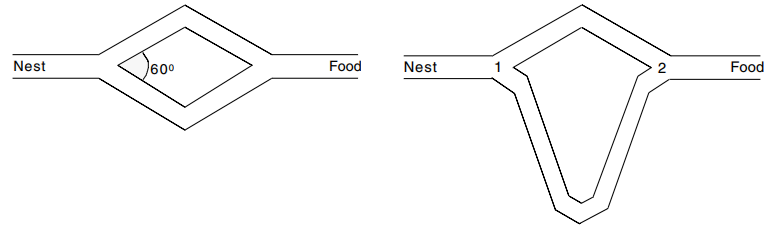
\includegraphics[width=\textwidth]{Figures/aco/double_bridge.png}
	\caption{The double bridge experiment. On the left, two bridges with the same length. Experimental results show that ants distribute themselves evenly amonst both bridges. 
On the right, one of the bridges is longer than the other. Experimental results show that ants use the shorter bridge more often.}
  \label{fig:double_bridge}  
\end{figure}

Using the model of a static combinatorial optimization problem, as defined in section \ref{sec:sec_2.1}, it is possible to derive a generic pheromone model that can be exploited by the Ant Colony Optimization. This means that both the classical and the time-dependent TSP, which can be formulated by the aforementioned model, may be solved by the ACO metaheuristic.
The following pseudo-code represents the algorithmic skeleton for the ACO model, and each of its parts will be explained with more detail below.


\makeatletter
\def\BState{\State\hskip-\ALG@thistlm}
\makeatother

\begin{algorithm}
\caption{ACO metaheuristic}\label{eq:aco_metacode}
\begin{algorithmic}[1]
\Procedure{AntColonyOptimization}{}
\State Initialization
\While{(termination condition not met)}
\State ConstructAntSolutions
\State ApplyLocalSearch \Comment{optional}
\State GlobalPheromonesUpdate
\EndWhile
\EndProcedure
\end{algorithmic}
\end{algorithm}


The general process of the Ant Colony Optimization algorithms is as follows. The algorithm starts with a parameter initialization. This is also responsible for setting the pheromones levels to some initial value $\tau_{0}$.
This value is usually chosen using a heuristic function. For the TSP case, the heuristic chosen is often the nearest neighbour.

After initialization, and until some specific termination condition is met, the ACO algorithm runs in a loop, which consists of 3 main steps: $i$)solution construction; $ii$)local search (optional); and $iii$) pheromone update. Each of this steps will be detailed below.

The solution construction is a process carried out by each of a specified number of ants. Each ant starts with an initially empty solution, $s_{p}$, and at each iteration step expands its solution with a valid solution component, $c_{i}^{j}$. This construction function is what differentiates the ACO algorithm for every combinatorial optimization problem. By restricting the construction method to the agents (the ants), the rest of the algorithm does not have to be heavily adapted to the specific model. However, the function that is responsible for selecting the feasible solution components has to be aware of the decision variables and the set of constraints. It has to determine those variables whose addition to the partial solution do not constitute a violation to the set of constraints of the model. This set is represented by $N(s_{p})$.

Having the set of all feasible solutions components, $N(s_{p})$, it is necessary to choose a single component, $c_{i}^{j}$. This selection is done probabilistically, and the choice takes into account both pheromone (exploitation) and heuristic information (exploration). The algorithmic parameter $q_{0}$ is responsible for defining both method's relative importance. The outline execution of the function is presented in equation \ref{eq:component_selection}, and is as follows. A random value, $q$, is set. If this value is lower than the algorithms parameter $q_{0}$, the selection of the node is done with the heuristic rule, equation \ref{eq:heuristic_rule}. Else, the Ant System rule, presented in \ref{eq:ant_system_rule}, is used.

\begin{equation} \label{eq:component_selection}
	c_{i}^{j} =
		\begin{cases}
			\textrm{heuristic rule}, \quad if q \leq q_{0} \\
			\textrm{ant system rule,} \quad \textrm{otherwise}
		\end{cases}
\end{equation}

\begin{equation} \label{eq:heuristic_rule}
	arg max_{l \in N_{i}^{k} } \tau_{il}[\eta_{il}]^{\beta}
\end{equation}


\begin{equation} \label{eq:ant_system_rule}
	p(c_{i}^{j}|s_{p}) = \frac{\tau_{ij}^{\alpha}  [\eta(c_{i}^{j})]^{\beta}}{\sum_{c_{i}^{l} \in N(s_{p})} \tau_{il}^{\alpha} [\eta(c_{i,l})]^{\beta}}
\end{equation}


After finalizing the construction of valid solutions, the ACO algorithm may implement a local search. Although this step is optional, it has been demonstrated that ACO algorithms reach their best performance when local search is applied. The ant's construction method is biased by the pheromone information, while the pheromones values are biased by the quality of the solutions. Local search, also called Daemon Actions, are techniques which intend to work on the existing solutions, exploring and expanding the search space, and ultimately improving the quality of the solutions. The most widely used local search methods are the 2-opt search, the 3-opt search, and the Lin-Kernighan heuristic.

The final step of each loop of the algorithm is the pheromone update, presented in equation \ref{eq:pheromone_update_rule}. This is responsible for making solution components that belong to good solutions more desirable in the following iterations. To achieve this objective, two methods are implemented. The first is pheromone deposition, which increases the pheromone intensity of the solution components belonging to the most promising solutions. The amount of solutions that are used to deposit pheromone is a parameter of the algorithm. The second method to achieve this step's goal, is pheromone evaporation. While it may seam counter-intuitive to deposit pheromones and, at the same time, also evaporate them, this step is crucial to avoid a rapid convergence to sub-optimal solutions. Pheromone deposition alone is responsible for making good solutions more desirable, while pheromone evaporation reduces both the desirability of bad solutions and the sub optimal convergence of good solutions, favoring the exploration of the search space. 

\begin{equation} \label{eq:pheromone_update_rule}
		\tau_{ij} = (1-\rho)\tau_{ij} + \sum_{s\in S_{upd}|c_{i}^{j}\in s}g(s)
\end{equation}